\documentclass[12pt,a4paper]{article}

% ===== PAKETE =====
\usepackage[ngerman]{babel}          % Deutsche Sprache
\usepackage[utf8]{inputenc}          % UTF-8 Kodierung
\usepackage[T1]{fontenc}             % Schriftkodierung
\usepackage{lmodern}                 % Schönere Schrift
\usepackage[left=2.5cm,right=2.5cm,top=2.5cm,bottom=2.5cm]{geometry}

% Layout & Formatierung
\usepackage{setspace}                % Zeilenabstand
\usepackage{parskip}                 % Absatzformatierung
\usepackage{fancyhdr}                % Kopf- und Fußzeilen

% Bilder & Grafiken
\usepackage{graphicx}                % Bilder einbinden
\usepackage{float}                   % Bessere Positionierung
\usepackage{caption}                 % Bildunterschriften

% Tabellen
\usepackage{tabularx}                % Flexible Tabellen
\usepackage{booktabs}                % Schönere Tabellen

% PDF einbinden
\usepackage{pdfpages}                % Für Deckblatt

% Mathematik (falls benötigt)
\usepackage{amsmath}
\usepackage{amssymb}

% Links & Verweise
\usepackage{hyperref}                % Klickbare Links
\hypersetup{
    colorlinks=true,
    linkcolor=black,
    citecolor=black,
    urlcolor=blue,
    pdftitle={Titel deiner Arbeit},
    pdfauthor={Dein Name}
}

% Literaturverzeichnis
\usepackage[backend=biber,style=numeric,sorting=none]{biblatex}
\addbibresource{literatur.bib}

% ===== EINSTELLUNGEN =====
\onehalfspacing                      % 1,5-facher Zeilenabstand
\setlength{\parindent}{0pt}          % Keine Einrückung

% Kopf- und Fußzeilen
\pagestyle{fancy}
\fancyhf{}
\fancyhead[L]{\leftmark}
\fancyhead[R]{\thepage}
\renewcommand{\headrulewidth}{0.4pt}

% ===== DOKUMENT =====
\begin{document}

% Vorgegebenes Deckblatt einbinden
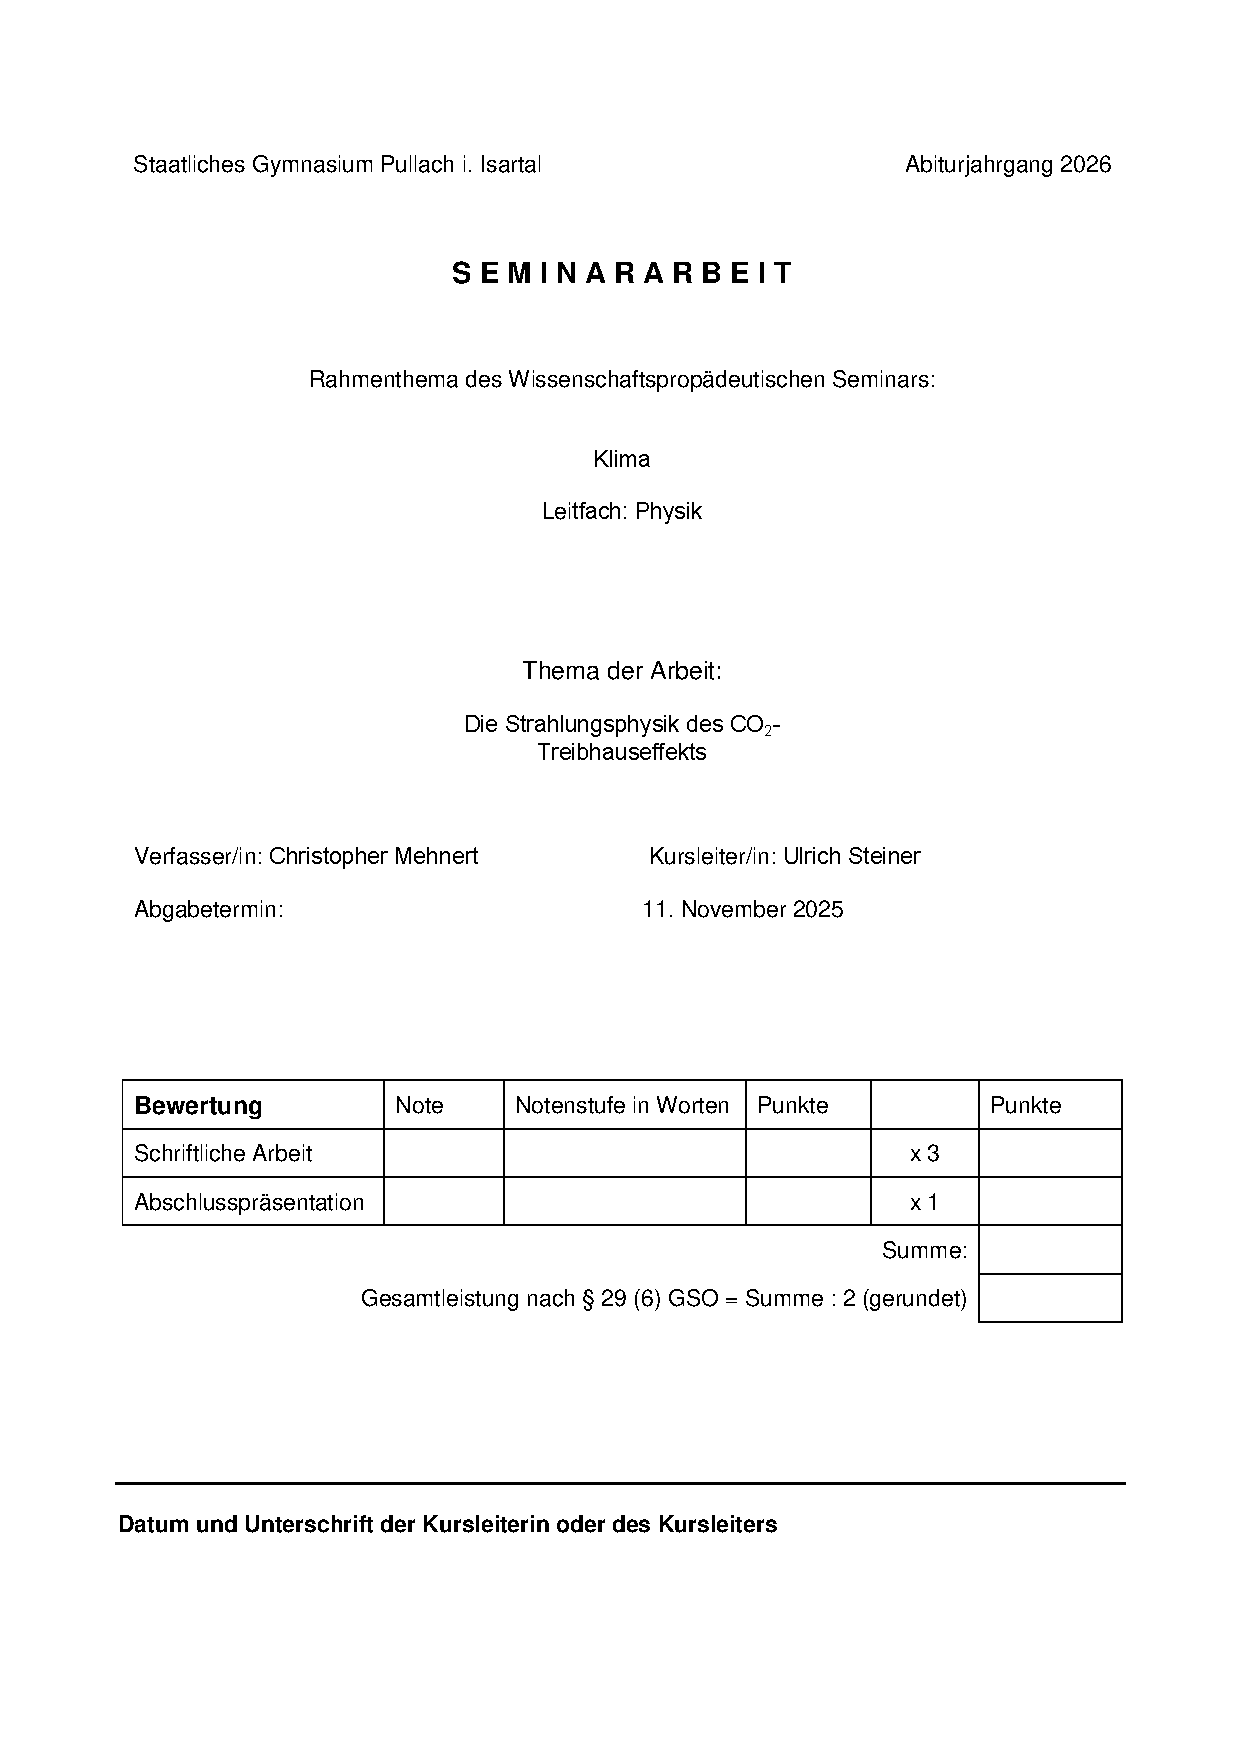
\includepdf[pages=1]{deckblatt.pdf}

% Römische Seitenzahlen für Verzeichnisse
\pagenumbering{roman}

% Inhaltsverzeichnis
\tableofcontents
\newpage

% Optional: Abbildungsverzeichnis
% \listoffigures
% \newpage

% Optional: Tabellenverzeichnis
% \listoftables
% \newpage

% Arabische Seitenzahlen für Hauptteil
\pagenumbering{arabic}

% ===== HAUPTTEIL =====

\section{Einleitung}
Hier kommt deine Einleitung...

\subsection{Motivation}
Warum ist das Thema relevant?

\subsection{Zielsetzung}
Was möchtest du erreichen?

\subsection{Aufbau der Arbeit}
Die Arbeit ist wie folgt strukturiert: ...


\section{Grundlagen}
Theoretischer Hintergrund...

\subsection{Begriffsdefinitionen}
Wichtige Begriffe erklären...

\subsection{Stand der Forschung}
Was wurde bereits erforscht? \cite{beispielquelle}


\section{Hauptteil}
Dein Kerninhalt...

\subsection{Methodik}
Wie bist du vorgegangen?

\subsection{Ergebnisse}
Was hast du herausgefunden?

% Beispiel: Bild einfügen
\begin{figure}[H]
    \centering
    \includegraphics[width=0.8\textwidth]{images/beispiel.png}
    \caption{Beschreibung des Bildes}
    \label{fig:beispiel}
\end{figure}

Wie in Abbildung \ref{fig:beispiel} zu sehen ist...

% Beispiel: Tabelle
\begin{table}[H]
    \centering
    \begin{tabularx}{0.8\textwidth}{l X}
        \toprule
        \textbf{Begriff} & \textbf{Beschreibung} \\
        \midrule
        Test 1 & Beschreibung 1 \\
        Test 2 & Beschreibung 2 \\
        \bottomrule
    \end{tabularx}
    \caption{Beispieltabelle}
    \label{tab:beispiel}
\end{table}


\section{Diskussion}
Interpretation der Ergebnisse...


\section{Fazit und Ausblick}
Zusammenfassung der wichtigsten Erkenntnisse...

\subsection{Zusammenfassung}
Die wesentlichen Punkte...

\subsection{Ausblick}
Mögliche zukünftige Forschung...


% ===== LITERATURVERZEICHNIS =====
\newpage
\printbibliography[title={Literaturverzeichnis}]

% ===== ANHANG (optional) =====
% \newpage
% \appendix
% \section{Zusätzliche Daten}
% ...

\end{document}